\documentclass{article}

% PACKAGES  ============================================================
\usepackage{lipsum}		% Used to generate dummy-text (\lipsum[1])
\usepackage[margin=2.54cm,includefoot]{geometry}		% Used to control margins
\usepackage{scrextend}	% To be able to use \begin{addmargin}

\usepackage{graphicx} % allows to import images
\usepackage{float}	% allows for control of float positions
\usepackage{tikz} 	% Used to create trees
\usepackage{pgfplots}	% to create plots

\usepackage{forest} % Used to create trees

\usepackage{amsmath}	 % to use cases in equations

\usepackage[hidelinks]{hyperref}	% allows for clickable references

\usepackage[numbers,sort&compress]{natbib} 	% sorts the cites in increasing order automatically when referenced and compresses successive references

\usepackage[utf8]{inputenc}		% Be able to use umlaute

\usepackage[ngerman]{babel}

\usepackage{fancyhdr}	% Used for Header and Footer stuff

\usepackage{xfrac}	% allows for slanted fractions 

\usepackage{pgfplots}	% Used for Linear regression plot

% ============================================================

% HEADER AND FOOTER STUFF ============================================================
\pagestyle{fancy}
\fancyhead{}	% clears header
\fancyfoot{}	% clears footer
\fancyfoot[R]{\thepage}	% sets position right
\renewcommand{\headrulewidth}{0pt}	% removes header line by setting it to zero
\renewcommand{\footrulewidth}{1pt}		% add footer line by setting it to one
% ============================================================

% DEFINE LIST ITEM BULLETS ============================================================
\renewcommand{\labelitemi}{$\bullet$}	% first list item
\renewcommand{\labelitemii}{$\circ$}	% one-indented item
\renewcommand{\labelitemiii}{$\diamond$}	% twice-indented item
% ============================================================


\begin{document}

% TITLE PAGE ============================================================
\begin{titlepage}
	
	\begin{center}
	\line(1,0){330} \\
	[2mm]
	\huge{\bfseries Data Science Zusammenfassung} \\
	[2mm]
	\line(1,0){320} \\
	[1,5cm]
	\textsc{\LARGE By Yannis Schmutz} \\
	[0.75cm]
	\textsc{\large todo} \\
	
	\end{center}
	
\end{titlepage}
% ============================================================

% PREFACE STUFF ============================================================
\pagenumbering{roman}		% sets the page numbering to roman for the preface etc.
\section*{Zusammenfassung}	% Adds a section without a number in front
\addcontentsline{toc}{section}{\numberline{}Zusammenfassung}	% adds a section without a number in front to the ToC
\cleardoublepage	% Finishes the current page so that the following page will always be odd.
% ****************************************************************

% TABLE OF CONTENTS ============================================================
\renewcommand{\contentsname}{Inhaltsverzeichnis}	% Rename table of contents to the german version
\tableofcontents		% adds table of contents (this needs to be compiled twice sometimes in order to update)
\thispagestyle{empty}	% removes header & footer on this page
\cleardoublepage	% Finishes the current page so that the following page will always be odd.
% ============================================================

% LIST OF FIGURES ============================================================
%\renewcommand{\listfigurename}{Abbildungsverzeichnis}	% renames list of figures
\listoffigures	% generates a list of figures
\addcontentsline{toc}{section}{Abbildungsverzeichnis}	% Adds list of figures to the ToC
\cleardoublepage
% ============================================================

% LIST OF TABLES ============================================================
%\renewcommand{\listtablename}{Tabellenverzeichnis}
\listoftables
\addcontentsline{toc}{section}{Tabellenverzeichnis}
\cleardoublepage
% ============================================================

% START OF REGULAR CHAPTERS ============================================================
\setcounter{page}{1}		% Sets this page to the first one (and not the table of contents)
\pagenumbering{arabic}	% Sets the page numbering back to arabic

\newpage
\section{Einleitung}
\label{sec:stat}


blub äöü
\newpage
\section{Statistik}
\label{sec:stat}

\subsection{Begriffe}
\begin{flushleft}
Dieses Kapitel bietet eine grobe �bersicht �ber einige hilfreiche Begriffe der Statistik.

\subsubsection{Lageparameter}
Lageparameter beschreiben die Lage der Stichprobenelemente im Bezug auf die Messskala.
\linebreak

\textbf{Mittelwert} \\
Auch Durchschnitt (oder mean im Englischen) gennant. In der Wahrscheinlichkeitsrechnung spricht man oft vom Erwartungswert.

$$\bar{x}_{arithm} = \frac{1}{n} \sum_{i=1}^{n} x_i$$

\textbf{Median} \\ 
Der Median oder auch Zentralwert genannt, beschreibt den Wert aus der auf-/ absteigend geordneten Stichprobe, der genau in der Mitte liegt.

\begin{equation*}
  \widetilde{x} = \begin{cases}
    x_{\frac{n+1}{2}}, & \text{\textit{n} ungerade}\\
    \frac{1}{2} \left( x_{\frac{n}{2}} + x_{\frac{n}{1}+1} \right), & \text{\textit{n} gerade}.
  \end{cases}
\end{equation*}


\textbf{Quantile} \\
Schwellenwert (engl. percentile) der angibt, dass ein bestimmter prozentualer Wert einer Menge an Werten kleiner ist als das Quantil. 
Das Quantil bei 50\% ist der Median. Weitere spezielle Quantile sind die Quartile, die Quintile, die Dezile und die Perzentile.
\linebreak

\textbf{Modus} \\
Definiert den h�ufigsten Wert, der in der Stichprobe vorkommt.


\subsubsection{Streuungsparameter}
Streuungsparameter beschreiben die Streuung von Werten einer Stichprobe um einen bestimmten Lageparameter. So ergeben sich je nach gew�hlten Lageparameter unterschiedliche Berechungsformen. Diese unterscheiden sich in ihrer Beeinflussung durch Ausreisser. So wird beispielsweise der Median tendenziell weniger von einem einzelnen, sehr hohen Ausreisser beeinflusst als der arithmetische Mittelwert.
\linebreak

\textbf{Spannweite} \\
Die Spannweite (eng. range) gibt den Abstand des gr�ssten gegen�ber dem kleinsten vorkommenden Wert der Stichprobe an. $R = x_{max} - x_{min}$.
\linebreak
Die Spannweite wird stark durch Ausreisser beeinflusst. Dem kann jedoch durch das alternative Verwenden des \textbf{Interquartilsabstands} (engl. interquartile range) entgegengewirkt werden. Dieser berechnet n�mlich die Spannweite zwischen zwei Quantilen. Somit k�nnen Ausreisser ignoriert werden.
\linebreak

\textbf{Varianz} \\
\linebreak






\textbf{Korrelation}
\linebreak


\textbf{Kovarianz}
\linebreak


\textbf{Kausalit�t}
\linebreak


\end{flushleft}


% ****************************************************************
\newpage
\section{Probabilistik}
\subsection{Bedingte Wahrscheinlichkeit}

Die bedingte Wahrscheinlichkeit ist die Wahrscheinlichkeit des Eintreten eines Ereignisses A unter der Bedingung, dass die Wahrscheinlichkeit für das Eintreten eines Ereignisses B bereits bekannt ist. Man spricht von \dq{A} unter der Bedingung B\dq. Oder auch $P(A|B)$.\\


Sind zwei Ereignisse E, F voneinander \textbf{unabhängig}, so gilt:
$$ P(E \cap F) = P(E)P(F) $$
$$ P(E|F) = P(E)$$

Sind jedoch zwei Ereignisse A, B \textbf{nicht unabhängig} so lautet die Formel für A unter der Bedingung B:
	$$P(A|B) = \frac{P(A \cap B)}{P(B)}$$


Daraus erschliesst sich:
	$$P(A \cap B) = P(A|B)P(B)$$


Das Aufzeichnen eines Wahrscheinlichkeitsbaumes hilft zur Veranschaulichung: \\

\begin{figure}[H]
	\centering
	\label{fig:probability_tree}
	\begin{forest}
	%\label{fig:probability_tree}
	for tree={circle,draw, s sep=3em}
	[ 
	    [$B$,edge label={node[midway,left] {$P(B)$}}
	      [$A \cap B$,edge label={node[midway,left] {$P(A|B)$}} ] 
	      [$\bar{A} \cap B$,edge label={node[midway,right] {$P(\bar{A}|B)$}}] 
	    ]
	    [$\bar{B}$,edge label={node[midway,right] {$P(\bar{B})$}}
	      [$A \cap \bar{B}$, edge label={node[midway,left] {$P(A|\bar{B})$}}] 
	      [$\bar{A} \cap \bar{B}$, edge label={node[midway,right] {$P(\bar{A}| \bar{B})$}}] 
	  ] 
	]
	\end{forest}
	\caption{Wahrscheinlichkeitsbaum}
\end{figure}

\subsubsection{Satz von Bayes}
%Verweis auf Kapitel \pageref{sec:stat}.

Der Satz von Bayes zeigt den Zusammenhang zwischen $P(A|B)$ und $P(B|A)$ auf:

\begin{equation}
\label{eq:bayes_theorem}
	P(A|B) = \frac{P(A \cap B)}{P(B)} = \frac{P(B|A)P(A)}{P(B)}
\end{equation}

Diese Gleichung \ref{eq:bayes_theorem} entsteht, wenn man den Ausdruck $P(A \cap B)$ anhand den umgekehrten Wahrscheinlichkeitsbaums \ref{fig:inv_probability_tree} ausdrückt. 


\begin{figure}[H]
	\centering
	\label{fig:inv_probability_tree}
	\begin{forest}
	for tree={circle,draw, s sep=3em}
	[ 
	    [$A$,edge label={node[midway,left] {$P(A)$}}
	      [$A \cap B$,edge label={node[midway,left] {$P(B|A)$}} ] 
	      [$A \cap \bar{B}$,edge label={node[midway,right] {$P(\bar{B}|A)$}}] 
	    ]
	    [$\bar{A}$,edge label={node[midway,right] {$P(\bar{A})$}}
	      [$\bar{A} \cap B$, edge label={node[midway,left] {$P(B|\bar{A})$}}] 
	      [$\bar{A} \cap \bar{B}$, edge label={node[midway,right] {$P(\bar{B}| \bar{A})$}}] 
	  ] 
	]
	\end{forest}
	\caption{Umgekehrter Wahrscheinlichkeitsbaum}
\end{figure}
% ****************************************************************


% ============================================================
\newpage
\section{Machine Learning}
\label{sec:ml}

\subsection{Übersicht}


\begin{figure}[H]
	\centering
	\label{fig:ml_overview}
	\begin{forest}
	for tree={draw, s sep=3em}
	[Machine Learning
	    [Überwachtes Lernen
	        [Klassifizierung
	            [Naive Bayes]
	             [k-N-N]
	             [NN]
	        ]
	        [Regression
	            [Linear Regression]
	            [NN]
	        ]
	    ]
	    [Unüberwachtes Lernen
	        [Clustering
	            [K-means]
	        ]
	        [Assoziierung]
	    ]
	]
	\end{forest}
	\caption{Machine Learning Kategorien}
\end{figure}

% #################################
\subsubsection{Überwachtes Lernen}
\begin{flushleft}

Überwachte Lern-Algorithmen probieren Beziehungen und Abhängigkeiten zwischen den Input-Features und des zu erzielenden Outputs zu erschliessen. Dies unter der Verwendung von \textbf{beschrifteten Daten}. Diese können zu Trainingszwecken verwendet werden. Jeder Satz an Daten besteht aus Input-Werten sowie einem dazugehörigen bekannten Output-Wert. Nach dem Trainieren des Algorithmus versucht dieser anhand von \textbf{neuen} Input-Features den dazugehörigen \textbf{unbekannten} Output vorherzusagen.
\linebreak

Das überwachte Lernen kann in zwei Kategorien unterteilt werden:

\begin{itemize}
	\item \textbf{Klassifizierung:} Ziel der Klassifizierung ist es, diskrete Werte vorherzusagen (bspw. Wahr/ Falsch, Spam-Mail/ normales Mail). 
	\item \textbf{Regression:} Das Ziel der Regression ist die Vorhersage kontinuierlicher Werte (bspw. Hauspreise in Abhängigkeit von Flaeche und Anzahl Zimmer).
\end{itemize}

\end{flushleft}

\subsubsection{Unueberwachtes Lernen}
\begin{flushleft}

Im unüberwachten Lernen stehen den Algorithmen \textbf{keine} beschrifteten Daten zur Verfügung. Die Algorithmen versuchen eigenständig Pattern in den zu behandelnden Daten zu erkennen und sie dadurch beispielsweise gruppieren zu können.
\end{flushleft}

% #################################

% ============================================================
\newpage
\section{Machine Learning Algorithmen}
\subsection{Linear Regression}

\begin{tikzpicture}
\begin{axis} [
	axis lines = left, % Only displays axis on left and bottom (not whole box)
	ymin = 0,	% y-axis shall always start at zero
	xlabel = $x$,
	ylabel = $f(x)$,
	mark=*,
	scatter/classes={%	Defines the point appearance for the scatter plot
		a={blue}%,
		%b={mark=triangle*,red},
		%c={mark=o,draw=black}
		}
	]

\addplot [
	domain = 0:60, 	% Range for the value x
	samples = 100,	% Determines the number of points in the interval defined by domain. 
	color = red,	% Color of the
	] {0.6*x + 10};
\addlegendentry {$mx + q$}

\addplot [only marks, scatter, scatter src=explicit symbolic]
	table [meta=class] {		% meta defines the column to use for the class of the point
		x		y		class
		10		20	a
		10		13		a
		20	20	a
		20	25		a
		30	26	a
		30	33	a
		40	33
		40	40
		50	44
		50	56
		60	40
	};

\end{axis}
\end{tikzpicture}



\subsection{Naive Bayes}

\begin{flushleft}
\end{flushleft}


% ============================================================


%\newpage
\section{Tryout}\label{sec:tryout}

\begin{figure}[H]	% H stands for here (place right here)
	\centering
	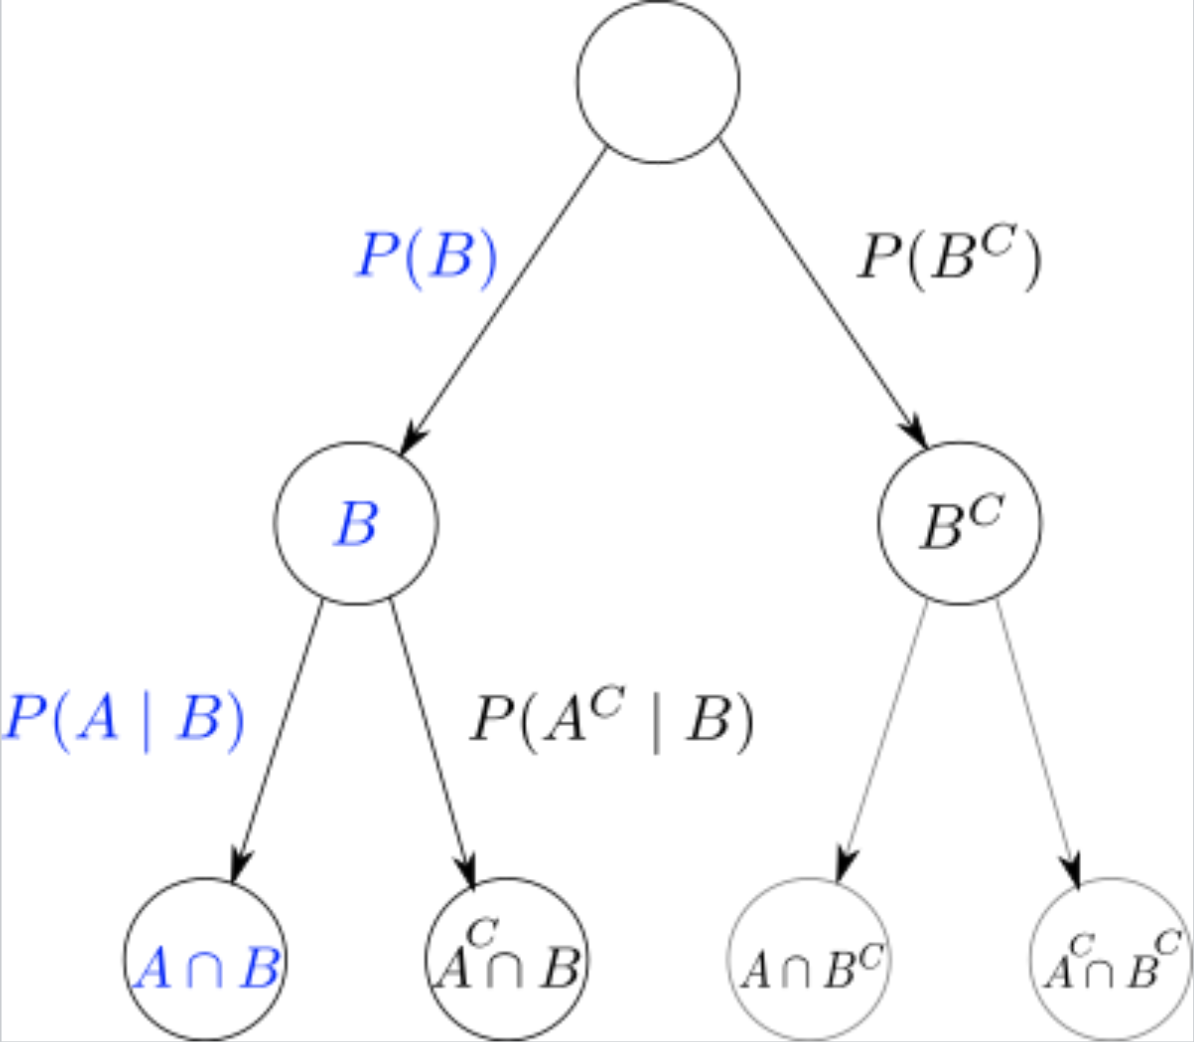
\includegraphics[height=5cm]{figures/tryout.png}
	\caption[Optional optional]{Entscheidungsbaum}
	\label{fig:tryout}
\end{figure}

Wie auf der Abbildung \ref{fig:tryout} zu sehen ist.....


\begin{table}[H]
	\centering
	\label{tab:tryouttab}
\caption[This is an optional caption, without reference]{Local caption, with reference}
	\cite{ref:ds_1, ref:nn_1, ref:ai_1}	% Used to add cites (zitieren)

	\begin{tabular}{l c r}
		Area & Number of rooms & Price \\ \hline
		80	& 4				& 1680 \\
		100	& 5				& 2300 \\
		50	& 2.5				& 1500 \\

	\end{tabular}
\end{table}


\begin{itemize}
	\item This is an item
	\item This is another item
	\begin{itemize}
		\item This is a further item
		\item [blub] This is an item with a custom bullet point
	\end{itemize}
\end{itemize}

\begin{enumerate}
	\item This is a numbered item
	\item And so on
\end{enumerate}


\newpage
\subsection{Math examples}

Here's an example within a sentence $E =mc^2$.

And here one example $$a=v/t$$ which is centred. \\

$$-\frac{\hbar^2}{2m}\frac{d^2\Psi}{dx^2} = E\Psi$$

Fractions

$$d = v_it + \frac{1}{2} \cdot at^2$$
$$d = v_it + \sfrac{1}{2} \cdot at^2$$


Brackets:
$$\left( \frac{1}{2} \right) \cdot 2 = 1$$	% use \left( ..... \right) to match the brackets to the content
$$\left| -7 \right| = 7$$
$$\sqrt{4} = 2$$
$$\sqrt{4} \ne 1$$
$$\sqrt{4} < 5$$
$$ \pi \approx 3 $$
$$ \pi \times \sqrt{4} < 15 $$

\begin{eqnarray}	% Equation array
	3x + 14 &=& 20 \\
	3x &=& 6 \\
	x &=& 2
\end{eqnarray}

\begin{equation}
\label{eq:first}
x^2 + 3x - 7 = 0
\end{equation}

\newpage
\subsection{Graphs}




\begin{tikzpicture}[sibling distance=12em,
							%root/.style={treenode,circle,draw},
							every child node/.style={circle, draw=black},
							]
%	[align=center, sibling distance=5cm]
	\node[fill=black]{}
		child { node {B}
		[sibling distance=6em]
			child { node{A $\cap$ B}  edge from parent node[left] {$P(A|B)$} }
			child { node{$\bar{A} \cap B$} edge from parent node[right] {$P(\bar{A}|B)$}}
			}
		child{ node{$\bar{B}$}
			[sibling distance=6em]
			child{ node{$A \cap \bar{B}$} edge from parent node[left] {$P(A|\bar{B})$}}
			child{ node{$\bar{A} \cap \bar{B}$} edge from parent node[right] {$P(\bar{A}|\bar{B})$} }
		       }
	;

\end{tikzpicture}
% ****************************************************************

% ============================================================




% REFERENCES ============================================================
\cleardoublepage
%\renewcommand{\bibname}{Referenzen}	% Rename the bibliography title
\bibliographystyle{IEEEtran}	% Adds cites (Zitate)
\addcontentsline{toc}{section}{Referenzen}
% references can easily be generated using the OS X tool "BibDesk"
% Make sure you build your LaTeX document in BibTeX after defining your references
%	in order to make them valid.
\bibliography{references/book_ref1}
% ============================================================

% APPENDIX ============================================================
\cleardoublepage
\appendix
\section{Cheatsheet}
% ============================================================


\end{document}